\section{Wechselstromtechnik}
	\subsection{Periodisch zeitabh\"angige Gr\"ossen}
 %		\subsubsection{Periodische Schwingungen}
 %			\begin{tabular}{p{6cm}p{4.5cm}p{7.5cm}}
 %				Frequenz &
 %           		\fbox{$f = \frac{1}{T} = \frac{2 \pi}{\omega}$} &
 %            		$[f] = s^{-1}$ \\ \\
 %				Schwingungsbreite &
 %					\fbox{$i_{pp} = i_{max} - i_{min}$} \\ \\
 %				Scheitelwert &
 %					\fbox{$\hat{i} = |i_{max}| \quad\text{für}\quad{|i_{max}|}\geq{|i_{min}|} \quad \text{oder} \quad \hat{i} = |i_{min}|\quad\text{für}\quad |i_{max}| < |i_{min}|$}
 %			\end{tabular}
		\subsubsection{Gleichrichterschaltungen}
			\begin{tabular}{p{4cm}p{4cm}p{9cm}}
            	\begin{minipage}{4cm}
            		\textbf{Einweggleichrichtung} \\
            		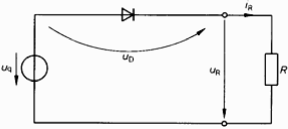
\includegraphics[height=1.2cm]{bilder/EinwegGleichrichtung.png}
            	\end{minipage} &
            		\begin{minipage}{4cm}
                    	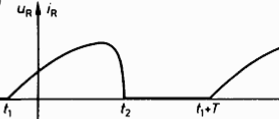
\includegraphics[width=4cm]{bilder/AusgangsspannungStromEinwegGleichrichtung.png}
                    \end{minipage} &
					\begin{minipage}{8cm}
                    	Fliesst nur ein Strom in Durchlassrichtung der Diode. \\
                    	Summe der Oberwellen $i_0=0.2176A$ \\
                    	$t_1 < t < t_2$ $\Rightarrow$ $u_R = u_q$ ; $i_R = u_q/R$ ; $u_D = 0$ \\
                    	$t_2 < t < (t_1+T)$ $\Rightarrow$ $u_R = 0$ ; $i_R = 0$ ; $u_D = u_q$
                    \end{minipage} \\
				\begin{minipage}{4cm}
                	\textbf{Zweiweggleichrichtung} \\
                	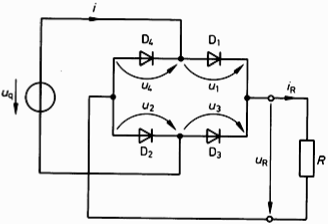
\includegraphics[height=1.5cm]{bilder/BrueckenGleichrichtung.png}
                \end{minipage} &
					\begin{minipage}{4cm}
                    	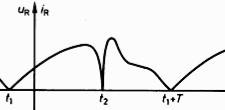
\includegraphics[width=4cm]{bilder/AusgangsspannungBrueckenGleichrichtung.png}
                    \end{minipage} &
					\begin{minipage}{9cm}
                    	Ausgangsspannung ist Betrag der Eingangsspannung. \\
                    	$t_1 < t < t_2$ $\Rightarrow$ $D_1,D_2$ leiten ; $D_3,D_4$ sperren \\
                    	$t_2 < t < (t_1+T)$ $\Rightarrow$ $D_1,D_2$ sperren ; $D_3,D_4$ leiten \\
                    	$u_R = |u_q|$ ; $i_R = u_R/R = |i|$
                    \end{minipage}
            \end{tabular}

		\subsubsection{Mittelwerte periodischer Gr\"ossen}
			\begin{tabular}{|p{5.5cm}|p{6cm}|p{6.5cm}|}
			\hline
				Arithmetischer Mittelwert, Gleichwert, Linearer MW &
				$X_0 = \overline{X} = X_m = \frac {1} {T} \int\limits_{t_0}^{t_0+T} x(t)dt$ &
				Ist die Fl\"ache unter der Zeitfunktion \"uber eine Periode. \\
			\hline
				Quadratischer MW, Leistung &
				$X^2 = \frac {1} {T} \int\limits_{t_0}^{t_0+T} x^2(t)dt$ & 
				$X^n = \frac {1} {T} \int\limits_{t_0}^{t_0+T} x^n(t)dt$ (MW $n$. Ordnung) \\
			\hline
				Effektivwert &
				$X = X_{\text{eff}}= \sqrt{X^2} = \sqrt{\frac{1}{T} \int\limits ^{t_0+T} _{t_0}{x^2(t)dt}}$
				& \\ 
			\hline
				Gleichrichtwert &
				$X_{|m|} = \bar{|X|} = \frac{1}{T} \int\limits_{t_0}^{t_0+T}{|x(t)| dt}$ &
				Arithm. Mittelwert der Zweiweggleichrichterschaltung \\
			\hline				    
				Energie der Periode $T$ &
				$W_T = \int\limits_{t_0}^{t_0+T}{P(t) dt} = \frac{X^2}{R}$ &
				ist die Energie positiv, nimmt der Zweipol Energie auf \\
			\hline                    
				Wirkleistung &
				$P = \frac{1}{T} \int\limits_{t_0}^{t_0+T}{P(t) dt}$ & \\
			\hline
			\end{tabular}
			
	\subsubsection{Verhältnisszahlen}
	\begin{multicols}{2}
	\begin{tabular}{ll}
	Scheitelfaktor $k_s$ (crest factor): & $k_s = \frac{\text{Scheitelwert}}{\text{Effektivwert}} = \frac{\hat{u}}{U}$ \\
    Formfaktor F (form factor): & $F = \frac{\text{Effektivwert}}{\text{Gleichrichtwert}} = \frac{U}{|\bar{u}|}$ \\	
	\end{tabular}
	\columnbreak
	
	\begin{tabular}{ll}
	Schwingungsgehalt: & $s = \frac{\text{Effektivwert des Wechselsignals}}{\text{Effektivwert der Mischgr\"osse}}$ \\
	Effektive Welligkeit: & $\frac{\text{Effektivwert des Wechselsignals}}{\text{Gleichwert der Mischgr\"osse}}$ \\
	Riffelfaktor: & $\frac{\text{Scheitelwert des Wechselsignals}}{\text{Gleichwert der Mischgr\"osse}}$ \\
	\end{tabular}
	\end{multicols}

			\begin{tabular}{p{5.5cm}p{5cm}p{7.5cm}}
				\textbf{Simpsonsche Regel}
				&	Gleichwert: &
						$\bar{i} = \frac{h}{3T} \sum m \cdot i$ \\ 
				\textit{(Berechnungsmethode anhand}		\\
				
				\textit{eines Graphen) }
				 &	Gleichrichtwert: &
						$|\bar{i}| = \frac{h}{3T} \sum m \cdot |i|$ \\ \\
						
				 &	Effektivwert: &
						$I_{eff} = \sqrt{\frac{h}{3T} \sum m \cdot i^2}$ \\ \\
				\begin{minipage}{4.5cm}
					\begin{tabular}{| c | c | c | c | c | c | c | c |}
						\hline
			 				$n$ & $t$ &$i$ & $i^2$ & $m$ & $m \cdot i$ & $m \cdot i^2$ \\
			 			\hline
				 			1 & & & & 1 & & \\
				 		\hline
				 			2 & & & & 2 & & \\
				 		\hline
				 			3 & & & & 4 & & \\
				 		\hline
				 			4 & & & & 2 & & \\
				 		\hline
				 			5 & & & & 1 & & \\
				 		\hline
			 		\end{tabular}
				\end{minipage} &
				\begin{minipage}{12.5cm}
                	W\"ahle im Graph der Aufgabenstellung, das den Strom i(t) darstellt, innerhalb
					der Periode $T$ eine ungerade Anzahl von $\boldsymbol{n}$ \textbf{Stützstellen} in konstanten
					\textbf{Abst\"anden }$\boldsymbol{h}=\frac{T}{n-1}$ (z.B $T=20ms, n=11$ mit $h=2 ms$). Lese an
					diesen Stellen jeweils den Augenblickswert des Stromes ab und tragen ihn in eine Tabelle ein (s.l). Berechne anschliessend für jede 
					Stützstelle den Wert von $i^2$ und den Summanden $m \cdot i^2$. Der \textbf{Faktor}
					$\boldsymbol{m}$ wird wie folgt gebildet: Für ungerade n ist m=4; bei der ersten und bei der
					letzten Stützstelle ist m=1, bei den übrigen ist m=2.
                \end{minipage}
			\end{tabular}
	\subsection{Sinusf\"ormige Schwingungen von Spannung und Strom}
% 		\subsubsection{Erzeugung sinusf\"ormiger Schwingungen}
% 			\begin{minipage}[t]{6cm}
%             	\textbf{Bewegte Leiter im \\ homogenen Magnetfeld}
%             \end{minipage}
% 			\begin{minipage}[lt]{4.5cm}
%             	$U = B \cdot l \cdot v$ \\
%             	$v_q = v \cdot cos\beta$ $\quad (v_p = v \cdot sin\beta)$ \\
%             	$U = \hat{U} \cdot sin\alpha$
%             \end{minipage}
% 			\begin{minipage}{3.5cm}
%             	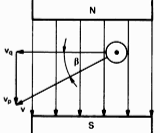
\includegraphics[width=3.5cm]{bilder/BewegteLeiter.png}
%             \end{minipage}
% 			\begin{minipage}{3.5cm}
%             	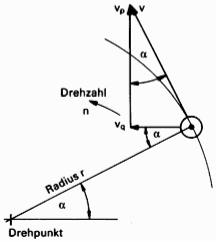
\includegraphics[width=3.5cm]{bilder/KreisfoermigeBewegung.png}
%             \end{minipage}
% 		\subsubsection{Beschreibung sinusf\"ormiger Spannungen und Str\"ome}
% 			\begin{tabular}{p{6cm}p{4.5cm}p{7.5cm}}
%             	\textbf{Kreisfrequenz} &
%             		\fbox{$\omega = \frac{2 \pi}{T} = 2 \pi f$} &
%             		$[\omega] = s^{-1}$ \\ \\
%             	\textbf{Effektivwert für sinusf\"ormige Gr\"ossen} &
%             		\fbox{$U = \frac{\hat{u}}{\sqrt{2}} \quad I = \frac{\hat{i}}{\sqrt{2}}$}
%             \end{tabular}
		\subsubsection{Komplexe Zeiger}
			\begin{minipage}[t]{6cm}
            	\textbf{Prinzip der Zeigertechnik}
            \end{minipage}
			\begin{minipage}{6cm}
            	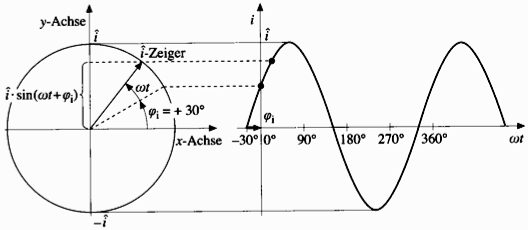
\includegraphics[width=6cm]{bilder/RotierenderScheitelwertzeiger.png}
            \end{minipage}
			\begin{minipage}{3.5cm}
            	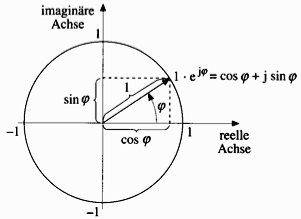
\includegraphics[width=3.5cm]{bilder/EulerscheRelation.png}
            \end{minipage} \\
			\begin{tabular}{p{5cm}p{4.5cm}p{8.5cm}}
            	Komplexer Effektivwert &
            		$\underline{U} = \frac{\underline{\hat{u}}}{\sqrt{2}}$ &
            		$\underline{U}$ = Kompl. Effektivwert, $\underline{\hat{u}}$ = Kompl. Scheitelwert \\
				Exponentialform &
					$\underline{\hat{u}} = \hat{u} \cdot e^{j\varphi_u} \quad \underline{U} = U \cdot e^{j\varphi_U}$ \\
				Algebraische Form &
					$\underline{\hat{u}} = \hat{u} (\cos(\varphi_u)+j\sin(\varphi_u))$ &
					$\Real(\underline{\hat{u}}) = \hat{u} \cdot \cos(\varphi_u)$ \quad $\Imag(\underline{\hat{u}}) = \hat{u} \cdot \sin(\varphi_u)$ \\
				&	$\underline{U} = U (\cos(\varphi_U)+j\sin(\varphi_U))$ &
					$\Real(\underline{U}) = U \cdot \cos(\varphi_U)$ \quad $\Imag(\underline{U}) = U \cdot \sin(\varphi_U)$ \\
				Umrechnung &
					$|\hat{u}| = \sqrt{\Real(\underline{\hat{u}})^2 + \Imag(\underline{\hat{u}})^2}$ \quad $\varphi_u = \arctan\left(\dfrac{\Imag(\underline{\hat{u}})}{\Real(\underline{\hat{u}})}\right)$ \\
				&	$|U| = \sqrt{\Real(\underline{U})^2 + \Imag(\underline{U})^2}$ \quad $\varphi_U = \arctan\left(\dfrac{\Imag(\underline{U})}{\Real(\underline{U})}\right)$ \\
				Komplexe Drehzeiger &
					$\underline{u}(t) = \underline{\hat{u}} \cdot e^{j\omega t} = \hat{u} \cdot e^{j\varphi_u} \cdot e^{j\omega t} = \hat{u} \cdot e^{j(\omega t + \varphi_u})$ \\
				Phasenwinkel &
					$\varphi = \varphi_u - \varphi_i$ &
					Phasenwinkel positiv $\rightarrow$ Spannung eilt Strom voraus (im Gegenuhrzeigersinn) \\
			\end{tabular}
		\subsubsection{Komponenten linearer Wechselstromnetzwerke}% \formelbuch{125}}
			\begin{tabular}{llll}
			$\underline{Z} = R +j X$: 
				& Komplexer Widerstand (Impedanz); 
				& $R$: Wirkwiderstand (Resistanz); 
				& $X$: Blindwiderstand (Reaktanz)\\
			$\underline{Y} = G + j B$: 
				& Komplexer Leitwert (Admittanz); 
				& $G$: Wirkleitwert (Konduktanz); 
				& $B$: Blindleitwert (Suszeptanz)
	      	\end{tabular} \\ \\
			\begin{tabular}{|l|l|l|l|l|}
			\hline
				\textbf{Widerstand} &
					$ \underline{Z_R} = R$ &
					$ \underline{Y} = G =\frac{1}{R}$ &
					&
					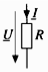
\includegraphics[height=1cm,angle=90]{bilder/Wirkwiderstand.png}
                	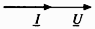
\includegraphics[width=1cm]{bilder/WirkwiderstandZeiger.png} \\
			\hline	                    
				\textbf{Induktivit\"at} &
					$ \underline{Z_L} = j \omega L = j X_L$&
					$ (X_L > 0) \quad \underline{Y_L} = - \frac{j}{\omega L} = j B_L$ &
					$W_L=\frac12 L I_L^2$ &
					
		            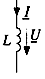
\includegraphics[height=1cm,angle=90]{bilder/Spule.png}
		            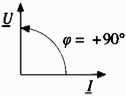
\includegraphics[width=1cm]{bilder/SpuleZeiger.png}
		            \\
			\hline		                
				\textbf{Kondensator} &
					$ \underline{Z_C} = \frac{1}{j \omega C} = - \frac{j}{\omega C} = - j
					X_C $ &
					$  (X_C < 0) \quad \underline{Y_C} = j \omega C = j B_C $&
					$W_C=\frac12 C U_C^2$ &
		            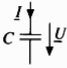
\includegraphics[height=0.8cm,angle=90]{bilder/Kondensator.png}
		            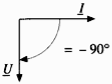
\includegraphics[width=1cm]{bilder/KondensatorZeiger.png}\\
			\hline	                
			\end{tabular}
		\subsubsection{Berechnung linearer Wechselstromnetzwerke}
		
		\subsubsection{Leistung im Wechselstromnetzwerk}% \formelbuch{162}}
				\begin{tabular}{p{4.5cm}p{7cm}p{7cm}}
					Komplexe Leistung &
						$ \underline{S} = \underline{U} \cdot \underline{I}^\ast = U\cdot I \cdot e^{j(\varphi_u-\varphi_i)}$   &
						Konjugiert Komplexer Strom! \\
					Wirkleistung [W] &
						$ P = \Real(\underline{S}) = U I \cos(\varphi) $ \\
					Blindleistung [var] &
						$ Q = \Imag(\underline{S}) = U I \sin(\varphi)  = P \cdot
						\tan\left(\varphi\right)$ & Kapazitiv: $Q < 0$; induktiv: $Q > 0$ \\
					Scheinleistung [VA] &
						$ S = | \underline{S} | = U I = \frac{U^2}{R} = I^2 R = \sqrt{P^2+Q^2}$ \\
					Leistungsfaktor &
						$\lambda = \frac{P}{S} = \frac{P}{UI} = \cos \varphi$ \\
				\end{tabular}
		\subsubsection{Blindleistungskompensation (mit Kondensator)}
		\renewcommand{\arraystretch}{1.5}
\begin{tabular}{p{7cm}p{4.5cm}p{5cm}}
	Kompensation mit C &
    	\begin{minipage}{4cm}
        	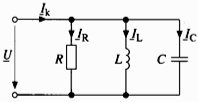
\includegraphics[width=3.5cm]{bilder/Parallelkompensation.png}
        \end{minipage} & 
		Der Kondensator wird parallel dazu geschalten \\ \\
	Zeigerdiagramme Kompensation &
		\begin{minipage}{4.5cm}
        	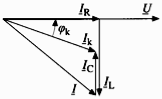
\includegraphics[width=3.5cm]{bilder/Blindstromkompensation.png}
        \end{minipage} &
		\begin{minipage}{4.5cm}
        	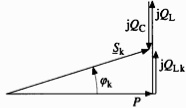
\includegraphics[width=3.5cm]{bilder/Blindleistungskompensation.png}
        \end{minipage} \\ \\
	Neue (kompensierte) Blindleistung &
		$Q_{Lk} = P \cdot \tan{\varphi_k}$ \\
	Blindleistung des Kondensators & 
		\multicolumn{2}{l}{$Q_C = Q_{Lk} - Q_L =  P\cdot (\tan{\varphi_k}-\tan{\varphi}) $} \\
	Kapazität des Kondensators &
		$C = - \frac{Q_C}{\omega U^2}$ \\	
	\end{tabular}
\renewcommand{\arraystretch}{1}
		\begin{multicols}{2}
			\subsubsection{RL Serieschaltung / Reihenschaltung}
				\begin{align*}
					P			&= \frac{U_R^2}{R_r}					& [W]		&= \frac{[V]}{[\Omega]}\\
					U_R			&= U_0 \cdot \cos\varphi				& [V]		& \\
					R_r			&= \frac{U_R^2}{P}						& [\Omega]	&= \frac{[V]^2}{[V A]} \\
					tan\varphi	&= \frac{\omega L_r}{R_r}				& 			& \\
					L_r			&= \frac{R_r \cdot tan\varphi}{\omega}	& [H]		&
				\end{align*}
			\columnbreak
			\subsubsection{RL Parallelschaltung}
				\begin{align*}
					P			&= \frac{U^2}{R_p}						& [W]		&= \frac{[V]}{[\Omega]}\\
					R_p			&= \frac{U^2}{P}						& [\Omega]	&= \frac{[V]^2}{[V A]} \\
					tan\varphi	&= \frac{R_p}{\omega L_p}				&			& \\
					L_p			&= \frac{R_p}{\omega \cdot \tan\varphi}	& [H]		& \\
					I_L			&= I_R \tan\varphi
				\end{align*}
		\end{multicols}

		\subsubsection{Leistungsumsatz bei nichtsinusf\"ormigen periodischen Gr\"ossen}
		\begin{minipage}[c]{7.5cm}
			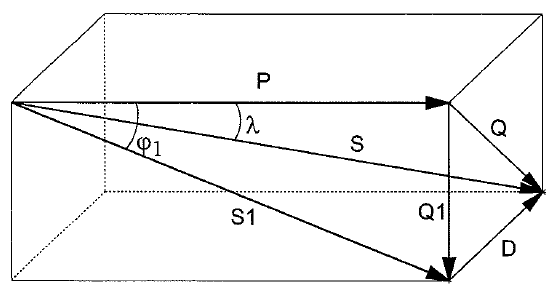
\includegraphics[height=4cm]{bilder/ZeigerdiagrammNichtSinus.png}     
    	\end{minipage}
		\begin{minipage}[c]{10.5cm}   
    		\noindent
    		\renewcommand{\arraystretch}{2.5}
    		\begin{tabular}{p{1.8cm} p{5.6cm}}
        		Unterwelle: 
        		& $X_{U} = \overline{X} = \dfrac{\hat{X}}{\sqrt{2}} a_0 \qquad $  \\
	     		Grundwelle: 
	     		& $X_{G} = \dfrac{\hat{X}}{\sqrt{2}} \sqrt{a_1^2 + b_1^2} \qquad  $   \\
	     		Oberwellen: 
	     		& $X_{O} = \dfrac{\hat{X}}{\sqrt{2}}
	     		\sqrt{\sum\limits_{k=2}^{\infty}a_k^2 +\sum\limits_{k=2}^{\infty}b_k^2}
	     		\qquad $  \\ \multicolumn{2}{l}{Effektivwerte: $X_{RMS} = \sqrt{X_G^2 + X_O^2} \qquad X_{TRMS} =
	     		\sqrt{X_U^2 + X_{RMS}^2}$ } \\
		\multicolumn{2}{l}{ges. Blindleistung: $Q = \sqrt{Q_G^2 + Q_U^2 + U^2
		\sum\limits_{k=2}^{\infty}I_k^2} = \sqrt{U^2 \sum\limits_{k=0}^{\infty}I_k^2}$} \\ 
		\multicolumn{2}{l}{Verzerrungsblindleistung: $D = U
		\cdot \sqrt{I_0^2 + \sum\limits_{k=2}^{\infty}I_k^2}$} \\
		\multicolumn{2}{l}{ges. Scheinleistung: $S = \sqrt{P^2 + Q^2 + D^2} = U \cdot I_{TRMS}$} \\
		 \end{tabular} \\
		 \renewcommand{\arraystretch}{1}
     	\end{minipage}    		\\ \\
     	Die Verzerrungsblindleistung wird von den Oberwellen und ev. von der Unterwelle (je
     	nach Phasenverschiebung) verursacht und ist mit Kondensatoren \textbf{nicht} zu kompensieren -
     	Aktive Filter w\"aren n\"otig.
		\\		
		
	\begin{minipage}[c]{8cm} 
	   \textbf{Beispiel anhand eines Einweggleichrichters:}	  	\\
	   (mit ohmscher Last R) 
	\end{minipage}   
	\begin{minipage}[c]{10cm} 	
	   $ \qquad i(t) = \underbrace{\frac{A}{\pi}}_{Unterwelle} + \underbrace{\frac{A}{2}
	   \sin(t)}_{Grundwelle} - \underbrace{\frac{2A}{\pi} \sum\limits_{k=1}^n \frac{1}{(2k-1)(2k+1)} \cos(2kt)}_{Oberwellen} $
	\end{minipage}   
		
	\begin{minipage}[c]{10cm}  
		\begin{tabular}{| l | l | l |}
    		\hline 
      		\textbf{Bezeichnung}
      		& \textbf{rel. Wert$^\ast$}
      		& \textbf{Formel} \\
      		\hline
      		Scheitelwert
      		& $\hat{I} = \sqrt{2} = 1,414$
      		& $= \hat{I}_d = \frac{\hat{U}_d}{R} $ \\
      		Mittelwert (DC)
      		& $I_m = 0.45$
      		& $= \bar{I}_d = \frac{\hat{I}}{\pi}$ \\
      		Grundwelle
      		& $I_G = 0.5$
      		& $= \frac{\hat{I}}{2 \cdot \sqrt{2}}$ \\
      		Oberwellen
      		& $I_O = 0.2162$
      		& $= \frac{\hat{I}}{\sqrt{2}} \cdot 0.21762$ \\
      		Effektivwert (AC)
      		& $I_{RMS} = 0.5433$
      		& $ = \sqrt{I_G^2 + i_O^2}$\\
      		True RMS
      		& $I_{TRMS} = 0.7071$
      		& $= \sqrt{I_m^2 + I_G^2 + i_O^2}$ \\
      		Laststrom
      		&
      		& $I_{d} =\frac{\hat{U}_s}{2 R}$ \\
      		Primärstrom
      		&
      		& $I_1 \approx I_U \cdot \frac{1.21}{"u}$ \\
      		Bauleistung 
      		&
      		& $S_{TR} = \frac{S_{1Tr} + S_{2Tr}}{2}$ \\
      		\hline 
    	\end{tabular} \newline
    	$^\ast$: bezogen auf $I_{Eff} = 1A$ im AC-Stromkreis ohne Diode
	\end{minipage}   
	\begin{minipage}[c]{8cm}  
			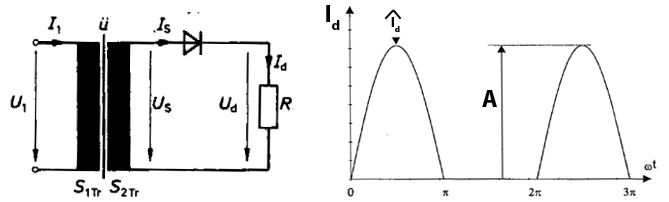
\includegraphics[width=8cm]{bilder/EinwegGR.png}  \\			
	$S_{1Tr} < S_{2Tr}$ da der Trafo keine Gleichstr\"ome übertr\"agt. Somit erscheint der Prim\"arstrom
	als Sekund\"arstrom mit unterdrücktem Gleichstromanteil.			
	\end{minipage}

	\begin{minipage}[c]{8cm} 
	   \textbf{Beispiel anhand eines Brückengleichrichters:}	  	\\
	   (mit ohmscher Last R)
	\end{minipage}   
	\begin{minipage}[c]{10cm} 	
	   $ \qquad i(t) = \underbrace{\frac{2A}{\pi}}_{Unterwelle} - \underbrace{\frac{4A}{\pi} \sum\limits_{k=1}^n \frac{1}{(2k-1)(2k+1)} \cos(2kt)}_{Oberwellen} $
	\end{minipage}\\
\begin{minipage}[c]{10cm}  
		\begin{tabular}{| l | l |}
    		\hline 
      		\textbf{Bezeichnung}
      		%& \textbf{N\"aherungsformel}
      		& \textbf{Formel} \\
      		\hline
      		Scheitelwert 
      		%& %& $\hat{I} = 0.7071 \cdot A $
      		& $\hat{I} = \hat{I}_d = \frac{\hat{U}_d}{R} $ \\
   %   		Fourien-Reihe
    %  		&$i(t)=A(\frac{2}{\pi}-\frac{4}{\pi}(\frac{\cos(2t)}{1\cdot
 %     		3}+\ldots+\frac{\cos(2nt)}{(2n-1) \cdot (2n+1)}))$\\
      		Unterwelle (Mittelwert)
      		%& $I_U = 0.22508 \cdot A $
      		& $I_U = \bar{I}_d = \frac{2 \hat{I}}{\pi}$ \\
      		Grundwelle
      		%& $I_G = 0.25 \cdot A$ 
      		& $I_G = 0$ \\
      		Oberwelle
      		%& $I_O = 0.10881 \cdot A$ 
      		& $I_O = \frac{\hat{I}}{\sqrt{2}} \cdot 0.43524$ \\
      		%Effektivwert (RMS)
      		%& $I_{RMS} = 0.27265 \cdot A$
      		%& $I_{RMS} = \sqrt{I_G^2 + I_O^2}$ \\ 
      		Laststrom
      		%& $I_{TRMS} = 0.35355 \cdot A$
      		& $I_{d eff} =  \frac{U_s}{R}= \frac{\hat{U}_d}{\sqrt{2}R}$ \\ 
      		Diodenstrom
      		& $I_{V} = \frac{\hat{U}}{2 R} = \frac{I_{d eff}}{\sqrt{2}}$ \\
      		Prim\"arstrom
      		& $I_1 \approx I_U \cdot \frac{0.966}{"u}$ \\
      		Bauleistung 
      		& $S_{TR} = \frac{S_{1Tr} + S_{2Tr}}{2}$ \\
      		\hline
    	\end{tabular}
	\end{minipage}   
	\begin{minipage}[c]{8cm}  
			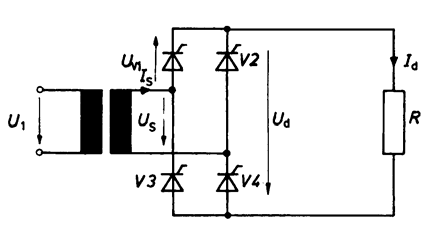
\includegraphics[width=7cm]{bilder/brueckengleichrichter.png}  \\			
	$S_{1Tr} < S_{2Tr}$ da der Trafo keine Gleichstr\"ome übertr\"agt. Somit erscheint der Prim\"arstrom
	als Sekund\"arstrom mit unterdrücktem Gleichstromanteil.			
	\end{minipage}
